\documentclass[%
	pdftex,
	a4paper,
	oneside,
%	twoside,
%	openany,
	bibtotoc,%	bib in die toc
	%~ makeidx,
	idxtotoc,%		index in die toc
	bibtotocnumbered,
	halfparskip,%         Europäischer Satz mit abstand zwischen Absätzen
%	chapterprefix,%
%	headsepline,%         Linie nach Kopfzeile
%	footsepline,%         Linie vor Fusszeile
%	12pt%                 Größere Schrift, besser lesbar am bildschrim
]{scrbook}
\usepackage[german, english]{babel} % greek for euro symbol with \textgreek{\euro}
%\usepackage{eurosans} % geht ned
\usepackage[german]{isodate} % dd.mm.yyyy
%\usepackage[latin1]{inputenc} % umlaute im quellcode
\usepackage[utf8]{inputenc}
\usepackage[T1]{fontenc} % umlaute im output als single chars
\usepackage{aeguill} % schöne (vektor?)schriften in verbindung mit umlauten
\usepackage[pdftex]{color,graphicx} % graphics import
\graphicspath{{./images/}}
\usepackage{epstopdf} % converts eps to automagically
%\epstopdfsetup{update,prepend,verbose} % does not work yet in ubuntu -> so wie rm all pdfs in the makefile
\usepackage{array} % mehr table options
\usepackage{booktabs} % \toprule \midrule \bottomrule etc
\usepackage{setspace}
\usepackage{amsmath} % für \begin{align} für multiline equations
\usepackage{amssymb}

\newcommand{\dokutitle}{AUA - Another Useless Architecture}

\usepackage[
	pdfauthor={grp4},
	pdftitle={\dokutitle},
	unicode=true,
	bookmarksnumbered=true,
	hyperindex=true,
	plainpages=false
]{hyperref} % underlined links
\hypersetup{
	colorlinks=true,	% false: boxed links; true: colored links
	linkcolor=black,	% color of internal links
	citecolor=black,	% color of links to bibliography
	filecolor=black,	% color of file links
	urlcolor=black,		% color of external links
	citebordercolor=0 0 0,	% hmpf!
	filebordercolor=0 0 0,
	linkbordercolor=0 0 0,
	menubordercolor=0 0 0,
	urlbordercolor=0 0 0,
	pdfborderstyle={/S/U/W 1},
	pdfstartview={FitV},
	bookmarksopen=true,
}
\usepackage{relsize}

\begin{document}
\chapter{Instruction Set Architecture}
\section{Registers}
\section{Instructions}
% \subsection{Addressing modes}
% \subsection{Special instructions}

\chapter{Assembler}
\section{Syntax}
\subsection{Example program}
\chapter{Pipeline stages}
blub

\begin{figure}[h!]
	\centerline { % relativ zur gesamten seite, fuer grosse figures!
	%~ \centering % relativ zur text area fuer figures <= textwidth
	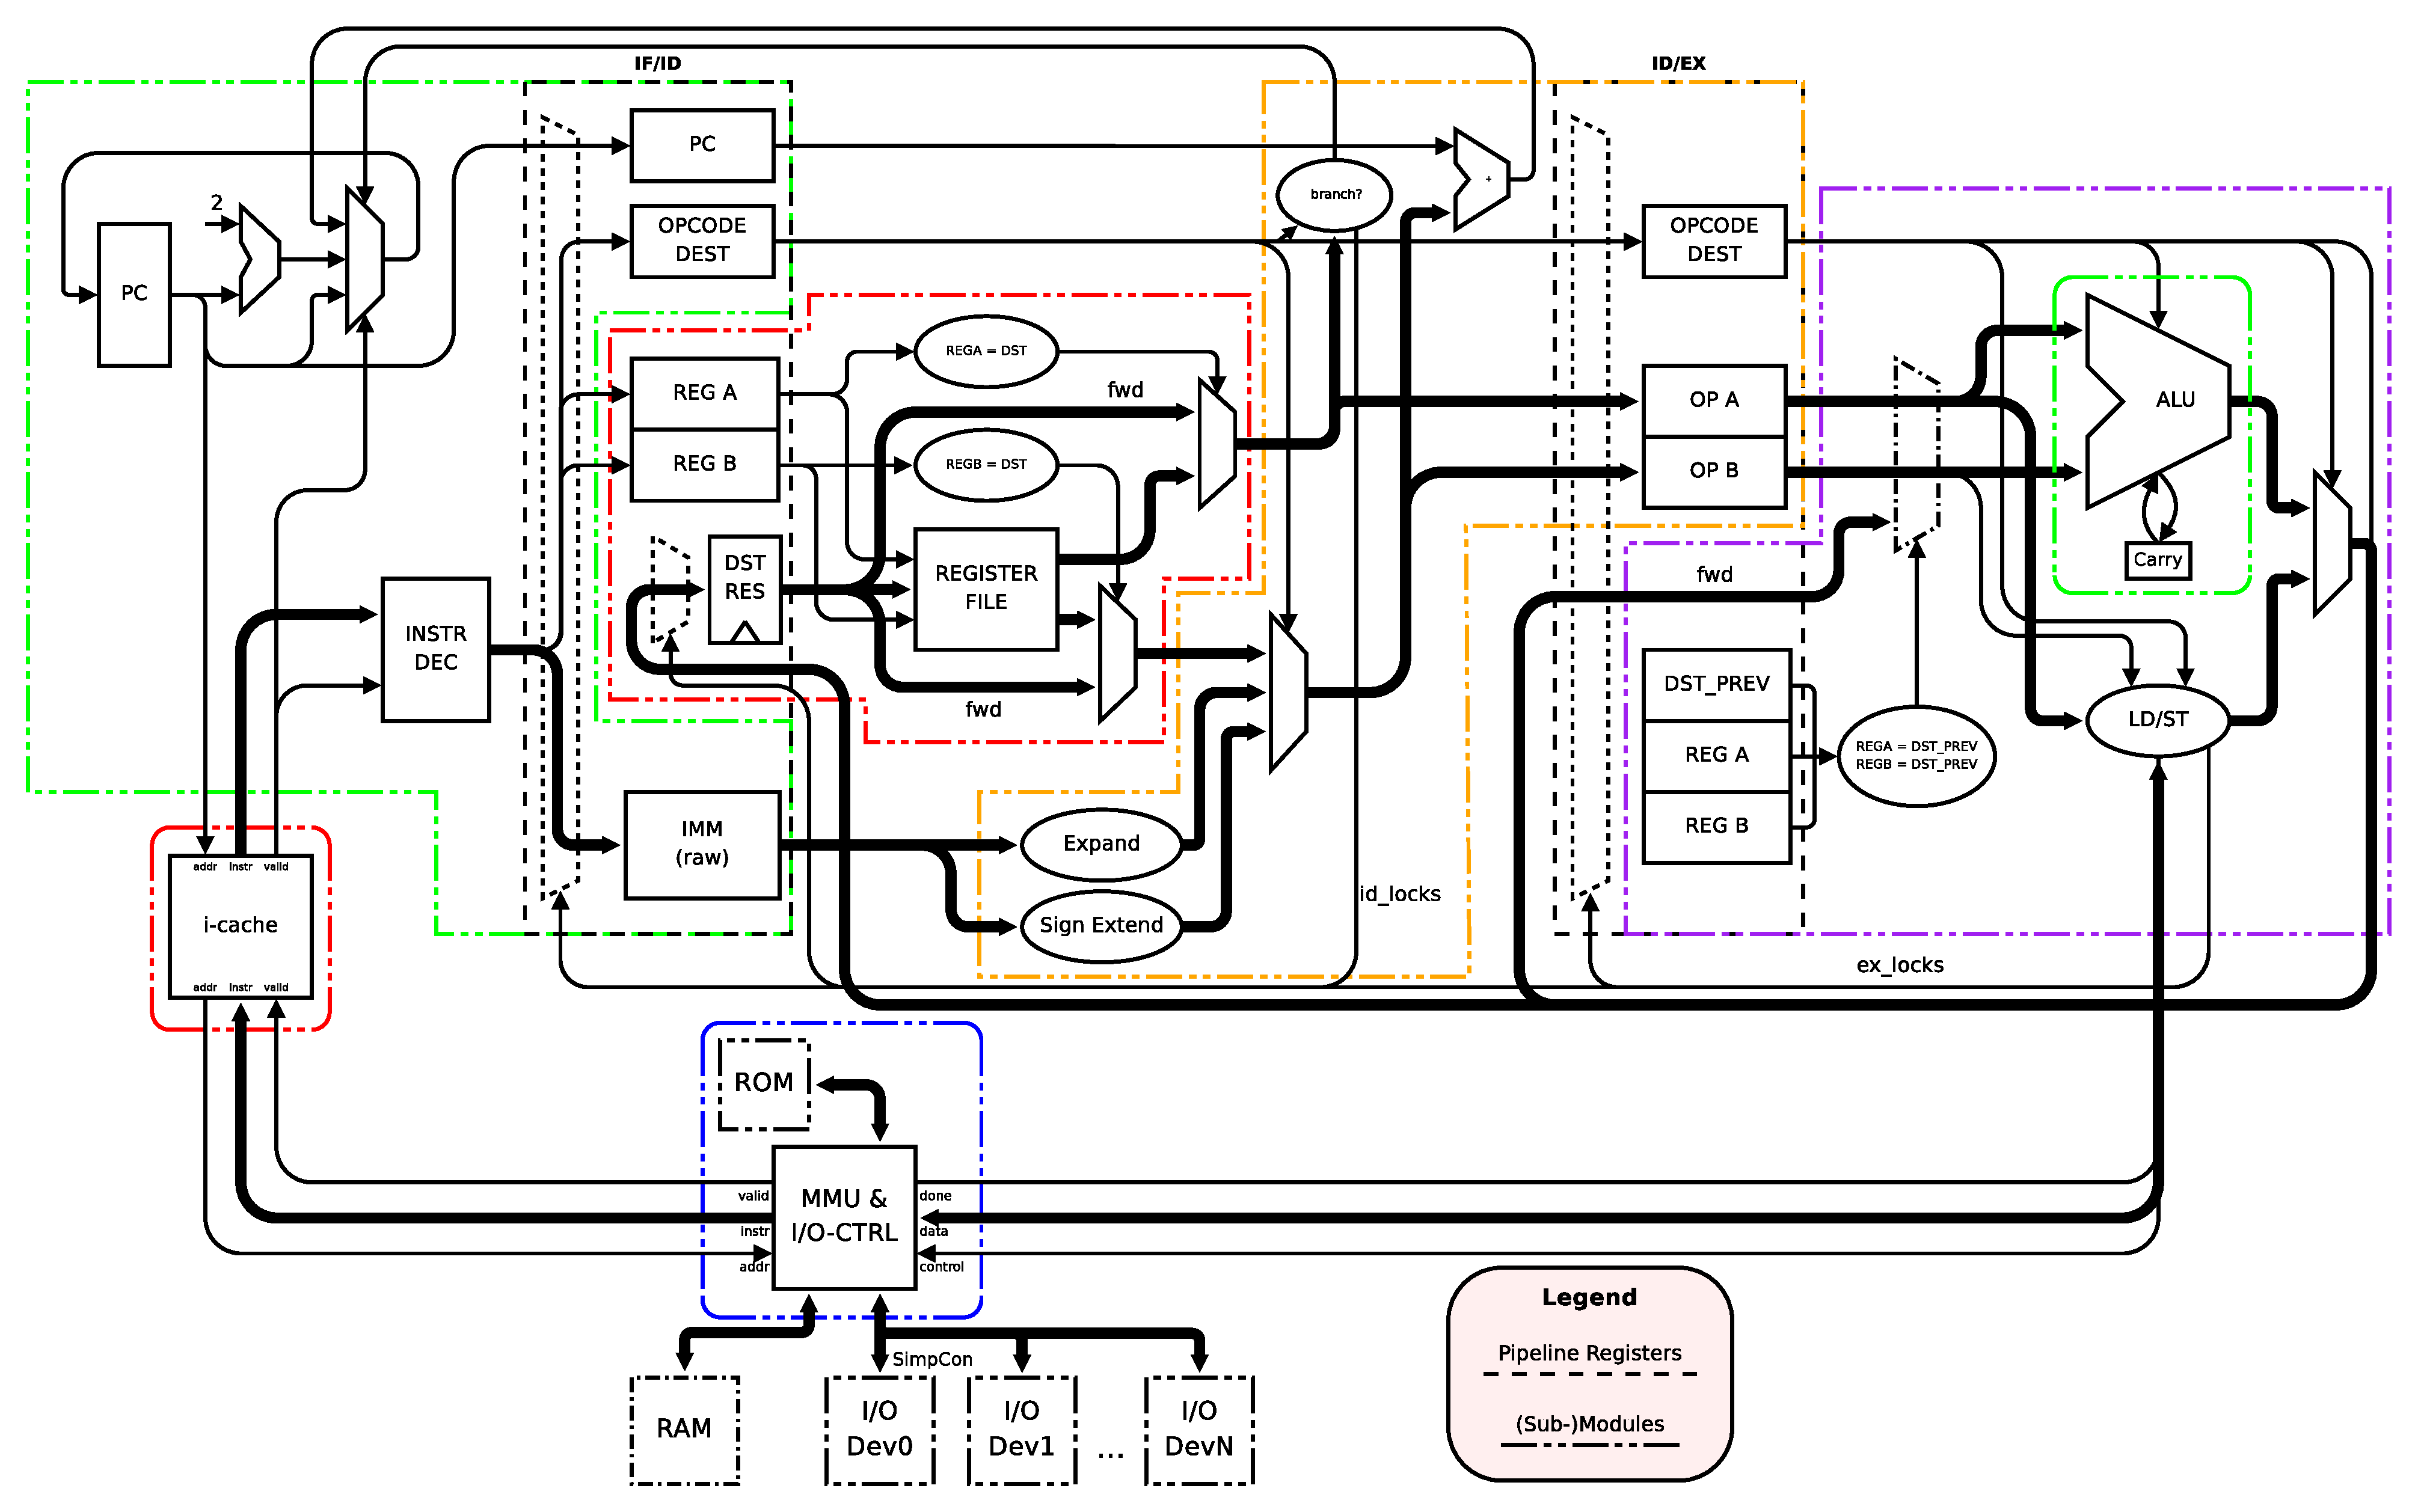
\includegraphics[width=1.2\textwidth]{schematic}
	}
	\caption[Schematic of the AUA pipeline]
	{Schematic of the AUA pipeline
	\label{label-schematic} }
\end{figure}

\chapter{rottiold}
\textbf{ldi - Load Immediate (signed)}

Description:

Load an 8 bit immediate to the register at bit 7 to 0

Immediate is 8 bits long and interpreted as signed

\begin{tabular}{|l|l|l|l|}
\hline
Operation & Syntax & Operands & Program Counter \\ \hline
Rd $\leftarrow $ Imm & LDI \ Rd, Imm &  &  \\ \hline
\end{tabular}

\begin{tabular}{|c|c|c|c|c|c|c|c|c|c|c|c|c|c|c|c|}
\hline
\multicolumn{6}{|l|}{Opcode} & \multicolumn{5}{|l|}{} & \multicolumn{5}{|l|}{
} \\ \hline
15 & 14 & 13 & 12 & 11 & 10 & 9 & 8 & 7 & 6 & 5 & 4 & 3 & 2 & 1 & 0 \\ \hline
0 & 0 & 0 & i & i & i & i & i & i & i & i & d & d & d & d & d \\ \hline
\end{tabular}

\bigskip

jmpl - Jump and Link

Description:

\begin{tabular}{|l|l|l|l|}
\hline
Operation & Syntax & Operands & Program Counter \\ \hline
PC $\longleftarrow $ Addr & JMPL \ \ Addr &  &  \\ \hline
\end{tabular}

\begin{tabular}{|c|c|c|c|c|c|c|c|c|c|c|c|c|c|c|c|}
\hline
\multicolumn{6}{|l|}{Opcode} & \multicolumn{5}{|l|}{} & \multicolumn{5}{|l|}{
} \\ \hline
15 & 14 & 13 & 12 & 11 & 10 & 9 & 8 & 7 & 6 & 5 & 4 & 3 & 2 & 1 & 0 \\ \hline
\multicolumn{1}{|l|}{0} & \multicolumn{1}{|l|}{0} & \multicolumn{1}{|l|}{1}
& \multicolumn{1}{|l|}{1} & \multicolumn{1}{|l|}{0} & \multicolumn{1}{|l|}{1}
& \multicolumn{1}{|l|}{a} & \multicolumn{1}{|l|}{a} & \multicolumn{1}{|l|}{a}
& \multicolumn{1}{|l|}{a} & \multicolumn{1}{|l|}{a} & \multicolumn{1}{|l|}{x}
& \multicolumn{1}{|l|}{x} & \multicolumn{1}{|l|}{x} & \multicolumn{1}{|l|}{x}
& \multicolumn{1}{|l|}{x} \\ \hline
\end{tabular}

\bigskip

brez - Branch if Equal Zero

Description:

\begin{tabular}{|l|l|l|l|}
\hline
Operation & Syntax & Operands & Program Counter \\ \hline
&  &  &  \\ \hline
\end{tabular}

\begin{tabular}{|c|c|c|c|c|c|c|c|c|c|c|c|c|c|c|c|}
\hline
\multicolumn{6}{|l|}{Opcode} & \multicolumn{5}{|l|}{} & \multicolumn{5}{|l|}{
} \\ \hline
15 & 14 & 13 & 12 & 11 & 10 & 9 & 8 & 7 & 6 & 5 & 4 & 3 & 2 & 1 & 0 \\ \hline
\multicolumn{1}{|l|}{0} & \multicolumn{1}{|l|}{0} & \multicolumn{1}{|l|}{1}
& \multicolumn{1}{|l|}{1} & \multicolumn{1}{|l|}{1} & \multicolumn{1}{|l|}{0}
& \multicolumn{1}{|l|}{a} & \multicolumn{1}{|l|}{a} & \multicolumn{1}{|l|}{a}
& \multicolumn{1}{|l|}{a} & \multicolumn{1}{|l|}{a} & \multicolumn{1}{|l|}{s}
& \multicolumn{1}{|l|}{s} & \multicolumn{1}{|l|}{s} & \multicolumn{1}{|l|}{s}
& \multicolumn{1}{|l|}{s} \\ \hline
\end{tabular}

\bigskip

brnez - Branch if Not Equal Zero

Description:

\begin{tabular}{|l|l|l|l|}
\hline
Operation & Syntax & Operands & Program Counter \\ \hline
&  &  &  \\ \hline
\end{tabular}

\begin{tabular}{|c|c|c|c|c|c|c|c|c|c|c|c|c|c|c|c|}
\hline
\multicolumn{6}{|l|}{Opcode} & \multicolumn{5}{|l|}{} & \multicolumn{5}{|l|}{
} \\ \hline
15 & 14 & 13 & 12 & 11 & 10 & 9 & 8 & 7 & 6 & 5 & 4 & 3 & 2 & 1 & 0 \\ \hline
\multicolumn{1}{|l|}{0} & \multicolumn{1}{|l|}{0} & \multicolumn{1}{|l|}{1}
& \multicolumn{1}{|l|}{1} & \multicolumn{1}{|l|}{1} & \multicolumn{1}{|l|}{1}
& \multicolumn{1}{|l|}{a} & \multicolumn{1}{|l|}{a} & \multicolumn{1}{|l|}{a}
& \multicolumn{1}{|l|}{a} & \multicolumn{1}{|l|}{a} & \multicolumn{1}{|l|}{s}
& \multicolumn{1}{|l|}{s} & \multicolumn{1}{|l|}{s} & \multicolumn{1}{|l|}{s}
& \multicolumn{1}{|l|}{s} \\ \hline
\end{tabular}

\bigskip

brezi - Branch if Equal Zero with Immediate

Description:

\begin{tabular}{|l|l|l|l|}
\hline
Operation & Syntax & Operands & Program Counter \\ \hline
&  &  &  \\ \hline
\end{tabular}

\begin{tabular}{|c|c|c|c|c|c|c|c|c|c|c|c|c|c|c|c|}
\hline
\multicolumn{6}{|l|}{Opcode} & \multicolumn{5}{|l|}{} & \multicolumn{5}{|l|}{
} \\ \hline
15 & 14 & 13 & 12 & 11 & 10 & 9 & 8 & 7 & 6 & 5 & 4 & 3 & 2 & 1 & 0 \\ \hline
\multicolumn{1}{|l|}{0} & \multicolumn{1}{|l|}{1} & \multicolumn{1}{|l|}{0}
& \multicolumn{1}{|l|}{0} & \multicolumn{1}{|l|}{i} & \multicolumn{1}{|l|}{i}
& \multicolumn{1}{|l|}{i} & \multicolumn{1}{|l|}{i} & \multicolumn{1}{|l|}{i}
& \multicolumn{1}{|l|}{i} & \multicolumn{1}{|l|}{i} & \multicolumn{1}{|l|}{s}
& \multicolumn{1}{|l|}{s} & \multicolumn{1}{|l|}{s} & \multicolumn{1}{|l|}{s}
& \multicolumn{1}{|l|}{s} \\ \hline
\end{tabular}

\bigskip

brnezi - Branch if Not Equal Zero with Immediate

Description:

\begin{tabular}{|l|l|l|l|}
\hline
Operation & Syntax & Operands & Program Counter \\ \hline
&  &  &  \\ \hline
\end{tabular}

\begin{tabular}{|c|c|c|c|c|c|c|c|c|c|c|c|c|c|c|c|}
\hline
\multicolumn{6}{|l|}{Opcode} & \multicolumn{5}{|l|}{} & \multicolumn{5}{|l|}{
} \\ \hline
15 & 14 & 13 & 12 & 11 & 10 & 9 & 8 & 7 & 6 & 5 & 4 & 3 & 2 & 1 & 0 \\ \hline
\multicolumn{1}{|l|}{0} & \multicolumn{1}{|l|}{1} & \multicolumn{1}{|l|}{0}
& \multicolumn{1}{|l|}{1} & \multicolumn{1}{|l|}{i} & \multicolumn{1}{|l|}{i}
& \multicolumn{1}{|l|}{i} & \multicolumn{1}{|l|}{i} & \multicolumn{1}{|l|}{i}
& \multicolumn{1}{|l|}{i} & \multicolumn{1}{|l|}{i} & \multicolumn{1}{|l|}{s}
& \multicolumn{1}{|l|}{s} & \multicolumn{1}{|l|}{s} & \multicolumn{1}{|l|}{s}
& \multicolumn{1}{|l|}{s} \\ \hline
\end{tabular}

\bigskip

\textbf{addi - Add Immediate}

Description:

Add an immediate to Rd and write the result back to Rd.

Immediate is 7 bit long and interpreted as signed.

\begin{tabular}{|l|l|l|l|}
\hline
Operation & Syntax & Operands & Program Counter \\ \hline
Rd $\leftarrow $ Rd + Imm & ADDI \ \ Rd, Imm &  &  \\ \hline
\end{tabular}

\begin{tabular}{|c|c|c|c|c|c|c|c|c|c|c|c|c|c|c|c|}
\hline
\multicolumn{6}{|l|}{Opcode} & \multicolumn{5}{|l|}{} & \multicolumn{5}{|l|}{
} \\ \hline
15 & 14 & 13 & 12 & 11 & 10 & 9 & 8 & 7 & 6 & 5 & 4 & 3 & 2 & 1 & 0 \\ \hline
\multicolumn{1}{|l|}{0} & \multicolumn{1}{|l|}{1} & \multicolumn{1}{|l|}{1}
& \multicolumn{1}{|l|}{0} & \multicolumn{1}{|l|}{i} & \multicolumn{1}{|l|}{i}
& \multicolumn{1}{|l|}{i} & \multicolumn{1}{|l|}{i} & \multicolumn{1}{|l|}{i}
& \multicolumn{1}{|l|}{i} & \multicolumn{1}{|l|}{i} & \multicolumn{1}{|l|}{d}
& \multicolumn{1}{|l|}{d} & \multicolumn{1}{|l|}{d} & \multicolumn{1}{|l|}{d}
& \multicolumn{1}{|l|}{d} \\ \hline
\end{tabular}

\bigskip

\textbf{muli - Multiply Immediate}

Description:

Multiply an immediate with Rd and write the result back to Rd

Immediate is 7 bit long and interpreted as signed.

\begin{tabular}{|l|l|l|l|}
\hline
Operation & Syntax & Operands & Program Counter \\ \hline
Rd $\leftarrow $ Rd x Imm & MULI \ \ Rd, Imm &  &  \\ \hline
\end{tabular}

\begin{tabular}{|c|c|c|c|c|c|c|c|c|c|c|c|c|c|c|c|}
\hline
\multicolumn{6}{|l|}{Opcode} & \multicolumn{5}{|l|}{} & \multicolumn{5}{|l|}{
} \\ \hline
15 & 14 & 13 & 12 & 11 & 10 & 9 & 8 & 7 & 6 & 5 & 4 & 3 & 2 & 1 & 0 \\ \hline
\multicolumn{1}{|l|}{0} & \multicolumn{1}{|l|}{1} & \multicolumn{1}{|l|}{1}
& \multicolumn{1}{|l|}{1} & \multicolumn{1}{|l|}{i} & \multicolumn{1}{|l|}{i}
& \multicolumn{1}{|l|}{i} & \multicolumn{1}{|l|}{i} & \multicolumn{1}{|l|}{i}
& \multicolumn{1}{|l|}{i} & \multicolumn{1}{|l|}{i} & \multicolumn{1}{|l|}{d}
& \multicolumn{1}{|l|}{d} & \multicolumn{1}{|l|}{d} & \multicolumn{1}{|l|}{d}
& \multicolumn{1}{|l|}{d} \\ \hline
\end{tabular}

\bigskip

\textbf{add - Add without carry}

Description:

Add two registers and write the result back to Rd

Carrybit is set, if an overflow occurrd

\begin{tabular}{|l|l|l|l|}
\hline
Operation & Syntax & Operands & Program Counter \\ \hline
Rd $\leftarrow $ Rd + Rs & ADD \ \ Rd, Rs &  &  \\ \hline
\end{tabular}

\begin{tabular}{|c|c|c|c|c|c|c|c|c|c|c|c|c|c|c|c|}
\hline
\multicolumn{6}{|l|}{Opcode} & \multicolumn{5}{|l|}{} & \multicolumn{5}{|l|}{
} \\ \hline
15 & 14 & 13 & 12 & 11 & 10 & 9 & 8 & 7 & 6 & 5 & 4 & 3 & 2 & 1 & 0 \\ \hline
\multicolumn{1}{|l|}{1} & \multicolumn{1}{|l|}{0} & \multicolumn{1}{|l|}{0}
& \multicolumn{1}{|l|}{0} & \multicolumn{1}{|l|}{0} & \multicolumn{1}{|l|}{0}
& \multicolumn{1}{|l|}{s} & \multicolumn{1}{|l|}{s} & \multicolumn{1}{|l|}{s}
& \multicolumn{1}{|l|}{s} & \multicolumn{1}{|l|}{s} & \multicolumn{1}{|l|}{d}
& \multicolumn{1}{|l|}{d} & \multicolumn{1}{|l|}{d} & \multicolumn{1}{|l|}{d}
& \multicolumn{1}{|l|}{d} \\ \hline
\end{tabular}

\bigskip

\textbf{addc - Add with Carry}

Description:

Add two registers and the Carrybit and write the result back to Rd

\begin{tabular}{|l|l|l|l|}
\hline
Operation & Syntax & Operands & Program Counter \\ \hline
Rd $\leftarrow $ Rd + Rs + C & ADDC \ \ Rd, Rs &  &  \\ \hline
\end{tabular}

\begin{tabular}{|c|c|c|c|c|c|c|c|c|c|c|c|c|c|c|c|}
\hline
\multicolumn{6}{|l|}{Opcode} & \multicolumn{5}{|l|}{} & \multicolumn{5}{|l|}{
} \\ \hline
15 & 14 & 13 & 12 & 11 & 10 & 9 & 8 & 7 & 6 & 5 & 4 & 3 & 2 & 1 & 0 \\ \hline
\multicolumn{1}{|l|}{1} & \multicolumn{1}{|l|}{0} & \multicolumn{1}{|l|}{0}
& \multicolumn{1}{|l|}{0} & \multicolumn{1}{|l|}{0} & \multicolumn{1}{|l|}{1}
& \multicolumn{1}{|l|}{s} & \multicolumn{1}{|l|}{s} & \multicolumn{1}{|l|}{s}
& \multicolumn{1}{|l|}{s} & \multicolumn{1}{|l|}{s} & \multicolumn{1}{|l|}{d}
& \multicolumn{1}{|l|}{d} & \multicolumn{1}{|l|}{d} & \multicolumn{1}{|l|}{d}
& \multicolumn{1}{|l|}{d} \\ \hline
\end{tabular}

\bigskip

\textbf{sub - Sub without carry}

Description:

Subtract two registers.and write the result back to Rd.

Carrybit is set, if an Underrun occurrd.

\begin{tabular}{|l|l|l|l|}
\hline
Operation & Syntax & Operands & Program Counter \\ \hline
Rd $\leftarrow $ Rd - Rs & SUB \ \ Rd, Rs &  &  \\ \hline
\end{tabular}

\begin{tabular}{|c|c|c|c|c|c|c|c|c|c|c|c|c|c|c|c|}
\hline
\multicolumn{6}{|l|}{Opcode} & \multicolumn{5}{|l|}{} & \multicolumn{5}{|l|}{
} \\ \hline
15 & 14 & 13 & 12 & 11 & 10 & 9 & 8 & 7 & 6 & 5 & 4 & 3 & 2 & 1 & 0 \\ \hline
\multicolumn{1}{|l|}{1} & \multicolumn{1}{|l|}{0} & \multicolumn{1}{|l|}{0}
& \multicolumn{1}{|l|}{0} & \multicolumn{1}{|l|}{1} & \multicolumn{1}{|l|}{0}
& \multicolumn{1}{|l|}{s} & \multicolumn{1}{|l|}{s} & \multicolumn{1}{|l|}{s}
& \multicolumn{1}{|l|}{s} & \multicolumn{1}{|l|}{s} & \multicolumn{1}{|l|}{d}
& \multicolumn{1}{|l|}{d} & \multicolumn{1}{|l|}{d} & \multicolumn{1}{|l|}{d}
& \multicolumn{1}{|l|}{d} \\ \hline
\end{tabular}

\bigskip

\textbf{subc - Sub with Carry}

Description:

Subtract tow regsiters and the carrybit and write the result back to Rd.

\begin{tabular}{|l|l|l|l|}
\hline
Operation & Syntax & Operands & Program Counter \\ \hline
Rd $\leftarrow $ Rd - Rs - C & SUB \ \ Rd, Rs &  &  \\ \hline
\end{tabular}

\begin{tabular}{|c|c|c|c|c|c|c|c|c|c|c|c|c|c|c|c|}
\hline
\multicolumn{6}{|l|}{Opcode} & \multicolumn{5}{|l|}{} & \multicolumn{5}{|l|}{
} \\ \hline
15 & 14 & 13 & 12 & 11 & 10 & 9 & 8 & 7 & 6 & 5 & 4 & 3 & 2 & 1 & 0 \\ \hline
\multicolumn{1}{|l|}{1} & \multicolumn{1}{|l|}{0} & \multicolumn{1}{|l|}{0}
& \multicolumn{1}{|l|}{0} & \multicolumn{1}{|l|}{1} & \multicolumn{1}{|l|}{1}
& \multicolumn{1}{|l|}{s} & \multicolumn{1}{|l|}{s} & \multicolumn{1}{|l|}{s}
& \multicolumn{1}{|l|}{s} & \multicolumn{1}{|l|}{s} & \multicolumn{1}{|l|}{d}
& \multicolumn{1}{|l|}{d} & \multicolumn{1}{|l|}{d} & \multicolumn{1}{|l|}{d}
& \multicolumn{1}{|l|}{d} \\ \hline
\end{tabular}

\bigskip

\textbf{mul - Multiply low word signed}

Description:

Multiply two registers and write the result back to Rd.

Registervalues are signed interpreted.

Result contains the low-word of the multiplication

\begin{tabular}{|l|l|l|l|}
\hline
Operation & Syntax & Operands & Program Counter \\ \hline
Rd $\leftarrow $ Rd x Rs & MUL \ \ Rd, Rs &  &  \\ \hline
\end{tabular}

\begin{tabular}{|c|c|c|c|c|c|c|c|c|c|c|c|c|c|c|c|}
\hline
\multicolumn{6}{|l|}{Opcode} & \multicolumn{5}{|l|}{} & \multicolumn{5}{|l|}{
} \\ \hline
15 & 14 & 13 & 12 & 11 & 10 & 9 & 8 & 7 & 6 & 5 & 4 & 3 & 2 & 1 & 0 \\ \hline
\multicolumn{1}{|l|}{1} & \multicolumn{1}{|l|}{0} & \multicolumn{1}{|l|}{0}
& \multicolumn{1}{|l|}{1} & \multicolumn{1}{|l|}{0} & \multicolumn{1}{|l|}{0}
& \multicolumn{1}{|l|}{s} & \multicolumn{1}{|l|}{s} & \multicolumn{1}{|l|}{s}
& \multicolumn{1}{|l|}{s} & \multicolumn{1}{|l|}{s} & \multicolumn{1}{|l|}{d}
& \multicolumn{1}{|l|}{d} & \multicolumn{1}{|l|}{d} & \multicolumn{1}{|l|}{d}
& \multicolumn{1}{|l|}{d} \\ \hline
\end{tabular}

\bigskip

\textbf{mulu - Multiply low word Unsigned}

Description:

Multiply two registers and write the result back to Rd.

Registervalues are unsigned interpreted.

Result contains the low-word of the multiplication

\begin{tabular}{|l|l|l|l|}
\hline
Operation & Syntax & Operands & Program Counter \\ \hline
Rd $\leftarrow $ Rd x Rs & MULU \ \ Rd, Rs &  &  \\ \hline
\end{tabular}

\begin{tabular}{|c|c|c|c|c|c|c|c|c|c|c|c|c|c|c|c|}
\hline
\multicolumn{6}{|l|}{Opcode} & \multicolumn{5}{|l|}{} & \multicolumn{5}{|l|}{
} \\ \hline
15 & 14 & 13 & 12 & 11 & 10 & 9 & 8 & 7 & 6 & 5 & 4 & 3 & 2 & 1 & 0 \\ \hline
\multicolumn{1}{|l|}{1} & \multicolumn{1}{|l|}{0} & \multicolumn{1}{|l|}{0}
& \multicolumn{1}{|l|}{1} & \multicolumn{1}{|l|}{0} & \multicolumn{1}{|l|}{1}
& \multicolumn{1}{|l|}{s} & \multicolumn{1}{|l|}{s} & \multicolumn{1}{|l|}{s}
& \multicolumn{1}{|l|}{s} & \multicolumn{1}{|l|}{s} & \multicolumn{1}{|l|}{d}
& \multicolumn{1}{|l|}{d} & \multicolumn{1}{|l|}{d} & \multicolumn{1}{|l|}{d}
& \multicolumn{1}{|l|}{d} \\ \hline
\end{tabular}

\bigskip

\textbf{mulh - Multiply High word signed}

Description:

Multiply two registers and write the result back to Rd.

Registervalues are signed interpreted.

Result contains the high-word of the multiplication.

\begin{tabular}{|l|l|l|l|}
\hline
Operation & Syntax & Operands & Program Counter \\ \hline
Rd $\leftarrow $ Rd x Rs & MULH \ \ Rd, Rs &  &  \\ \hline
\end{tabular}

\begin{tabular}{|c|c|c|c|c|c|c|c|c|c|c|c|c|c|c|c|}
\hline
\multicolumn{6}{|l|}{Opcode} & \multicolumn{5}{|l|}{} & \multicolumn{5}{|l|}{
} \\ \hline
15 & 14 & 13 & 12 & 11 & 10 & 9 & 8 & 7 & 6 & 5 & 4 & 3 & 2 & 1 & 0 \\ \hline
\multicolumn{1}{|l|}{1} & \multicolumn{1}{|l|}{0} & \multicolumn{1}{|l|}{0}
& \multicolumn{1}{|l|}{1} & \multicolumn{1}{|l|}{1} & \multicolumn{1}{|l|}{0}
& \multicolumn{1}{|l|}{s} & \multicolumn{1}{|l|}{s} & \multicolumn{1}{|l|}{s}
& \multicolumn{1}{|l|}{s} & \multicolumn{1}{|l|}{s} & \multicolumn{1}{|l|}{d}
& \multicolumn{1}{|l|}{d} & \multicolumn{1}{|l|}{d} & \multicolumn{1}{|l|}{d}
& \multicolumn{1}{|l|}{d} \\ \hline
\end{tabular}

\bigskip

\textbf{mulhu - Multiply High word Unsigned}

Description:

Multiply two registers and write the result back to Rd.

Registervalues are unsigned interpreted.

Result contains the high-word of the multiplication

\begin{tabular}{|l|l|l|l|}
\hline
Operation & Syntax & Operands & Program Counter \\ \hline
Rd $\leftarrow $ Rd x Rs & MULHU \ \ Rd, Rs &  &  \\ \hline
\end{tabular}

\begin{tabular}{|c|c|c|c|c|c|c|c|c|c|c|c|c|c|c|c|}
\hline
\multicolumn{6}{|l|}{Opcode} & \multicolumn{5}{|l|}{} & \multicolumn{5}{|l|}{
} \\ \hline
15 & 14 & 13 & 12 & 11 & 10 & 9 & 8 & 7 & 6 & 5 & 4 & 3 & 2 & 1 & 0 \\ \hline
\multicolumn{1}{|l|}{1} & \multicolumn{1}{|l|}{0} & \multicolumn{1}{|l|}{0}
& \multicolumn{1}{|l|}{1} & \multicolumn{1}{|l|}{1} & \multicolumn{1}{|l|}{1}
& \multicolumn{1}{|l|}{s} & \multicolumn{1}{|l|}{s} & \multicolumn{1}{|l|}{s}
& \multicolumn{1}{|l|}{s} & \multicolumn{1}{|l|}{s} & \multicolumn{1}{|l|}{d}
& \multicolumn{1}{|l|}{d} & \multicolumn{1}{|l|}{d} & \multicolumn{1}{|l|}{d}
& \multicolumn{1}{|l|}{d} \\ \hline
\end{tabular}

\bigskip

\textbf{or - Logical Or}

Description:

Bitwise or combination of the two registers.

Result write back to Rd

\begin{tabular}{|l|l|l|l|}
\hline
Operation & Syntax & Operands & Program Counter \\ \hline
Rd $\leftarrow $ Rd $\vee $ Rs & OR \ \ Rd, Rs &  &  \\ \hline
\end{tabular}

\begin{tabular}{|c|c|c|c|c|c|c|c|c|c|c|c|c|c|c|c|}
\hline
\multicolumn{6}{|l|}{Opcode} & \multicolumn{5}{|l|}{} & \multicolumn{5}{|l|}{
} \\ \hline
15 & 14 & 13 & 12 & 11 & 10 & 9 & 8 & 7 & 6 & 5 & 4 & 3 & 2 & 1 & 0 \\ \hline
\multicolumn{1}{|l|}{1} & \multicolumn{1}{|l|}{0} & \multicolumn{1}{|l|}{1}
& \multicolumn{1}{|l|}{0} & \multicolumn{1}{|l|}{0} & \multicolumn{1}{|l|}{0}
& \multicolumn{1}{|l|}{s} & \multicolumn{1}{|l|}{s} & \multicolumn{1}{|l|}{s}
& \multicolumn{1}{|l|}{s} & \multicolumn{1}{|l|}{s} & \multicolumn{1}{|l|}{d}
& \multicolumn{1}{|l|}{d} & \multicolumn{1}{|l|}{d} & \multicolumn{1}{|l|}{d}
& \multicolumn{1}{|l|}{d} \\ \hline
\end{tabular}

\bigskip

\textbf{and - Logical And}

Description:

Bitwise and combination of the two registers.

Result write back to Rd.

\begin{tabular}{|l|l|l|l|}
\hline
Operation & Syntax & Operands & Program Counter \\ \hline
Rd $\leftarrow $ Rd $\wedge $ Rs & AND\ \ \ Rd, Rs &  &  \\ \hline
\end{tabular}

\begin{tabular}{|c|c|c|c|c|c|c|c|c|c|c|c|c|c|c|c|}
\hline
\multicolumn{6}{|l|}{Opcode} & \multicolumn{5}{|l|}{} & \multicolumn{5}{|l|}{
} \\ \hline
15 & 14 & 13 & 12 & 11 & 10 & 9 & 8 & 7 & 6 & 5 & 4 & 3 & 2 & 1 & 0 \\ \hline
\multicolumn{1}{|l|}{1} & \multicolumn{1}{|l|}{0} & \multicolumn{1}{|l|}{1}
& \multicolumn{1}{|l|}{0} & \multicolumn{1}{|l|}{0} & \multicolumn{1}{|l|}{1}
& \multicolumn{1}{|l|}{s} & \multicolumn{1}{|l|}{s} & \multicolumn{1}{|l|}{s}
& \multicolumn{1}{|l|}{s} & \multicolumn{1}{|l|}{s} & \multicolumn{1}{|l|}{d}
& \multicolumn{1}{|l|}{d} & \multicolumn{1}{|l|}{d} & \multicolumn{1}{|l|}{d}
& \multicolumn{1}{|l|}{d} \\ \hline
\end{tabular}

\bigskip

\textbf{xor - Logical xor}

Description:

Bitwise xor combination of the two registers.

Result write back to Rd.

\begin{tabular}{|l|l|l|l|}
\hline
Operation & Syntax & Operands & Program Counter \\ \hline
Rd $\leftarrow $ Rd $\oplus $ Rs & XOR \ \ Rd, Rs &  &  \\ \hline
\end{tabular}

\begin{tabular}{|c|c|c|c|c|c|c|c|c|c|c|c|c|c|c|c|}
\hline
\multicolumn{6}{|l|}{Opcode} & \multicolumn{5}{|l|}{} & \multicolumn{5}{|l|}{
} \\ \hline
15 & 14 & 13 & 12 & 11 & 10 & 9 & 8 & 7 & 6 & 5 & 4 & 3 & 2 & 1 & 0 \\ \hline
\multicolumn{1}{|l|}{1} & \multicolumn{1}{|l|}{0} & \multicolumn{1}{|l|}{1}
& \multicolumn{1}{|l|}{0} & \multicolumn{1}{|l|}{1} & \multicolumn{1}{|l|}{0}
& \multicolumn{1}{|l|}{s} & \multicolumn{1}{|l|}{s} & \multicolumn{1}{|l|}{s}
& \multicolumn{1}{|l|}{s} & \multicolumn{1}{|l|}{s} & \multicolumn{1}{|l|}{d}
& \multicolumn{1}{|l|}{d} & \multicolumn{1}{|l|}{d} & \multicolumn{1}{|l|}{d}
& \multicolumn{1}{|l|}{d} \\ \hline
\end{tabular}

\bigskip

\textbf{not - Invert }

Description:

Invert the bits of register Rd, and write the result back to Rd.

\begin{tabular}{|l|l|l|l|}
\hline
Operation & Syntax & Operands & Program Counter \\ \hline
Rd $\leftarrow $ not Rd & NOT \ \ Rd &  &  \\ \hline
\end{tabular}

\begin{tabular}{|c|c|c|c|c|c|c|c|c|c|c|c|c|c|c|c|}
\hline
\multicolumn{6}{|l|}{Opcode} & \multicolumn{5}{|l|}{} & \multicolumn{5}{|l|}{
} \\ \hline
15 & 14 & 13 & 12 & 11 & 10 & 9 & 8 & 7 & 6 & 5 & 4 & 3 & 2 & 1 & 0 \\ \hline
\multicolumn{1}{|l|}{1} & \multicolumn{1}{|l|}{0} & \multicolumn{1}{|l|}{1}
& \multicolumn{1}{|l|}{0} & \multicolumn{1}{|l|}{1} & \multicolumn{1}{|l|}{1}
& \multicolumn{1}{|l|}{s} & \multicolumn{1}{|l|}{s} & \multicolumn{1}{|l|}{s}
& \multicolumn{1}{|l|}{s} & \multicolumn{1}{|l|}{s} & \multicolumn{1}{|l|}{d}
& \multicolumn{1}{|l|}{d} & \multicolumn{1}{|l|}{d} & \multicolumn{1}{|l|}{d}
& \multicolumn{1}{|l|}{d} \\ \hline
\end{tabular}

\bigskip

\textbf{neg - Negate}

Description:

Calculate the 2'es complement of Rd and write the result back to Rd.

Max value 0xFFFF left unchanged.

\begin{tabular}{|l|l|l|l|}
\hline
Operation & Syntax & Operands & Program Counter \\ \hline
Rd $\leftarrow \pm $ Rd & NEG \ \ Rd &  &  \\ \hline
\end{tabular}

\begin{tabular}{|c|c|c|c|c|c|c|c|c|c|c|c|c|c|c|c|}
\hline
\multicolumn{6}{|l|}{Opcode} & \multicolumn{5}{|l|}{} & \multicolumn{5}{|l|}{
} \\ \hline
15 & 14 & 13 & 12 & 11 & 10 & 9 & 8 & 7 & 6 & 5 & 4 & 3 & 2 & 1 & 0 \\ \hline
\multicolumn{1}{|l|}{1} & \multicolumn{1}{|l|}{0} & \multicolumn{1}{|l|}{1}
& \multicolumn{1}{|l|}{1} & \multicolumn{1}{|l|}{0} & \multicolumn{1}{|l|}{0}
& \multicolumn{1}{|l|}{s} & \multicolumn{1}{|l|}{s} & \multicolumn{1}{|l|}{s}
& \multicolumn{1}{|l|}{s} & \multicolumn{1}{|l|}{s} & \multicolumn{1}{|l|}{d}
& \multicolumn{1}{|l|}{d} & \multicolumn{1}{|l|}{d} & \multicolumn{1}{|l|}{d}
& \multicolumn{1}{|l|}{d} \\ \hline
\end{tabular}

\bigskip

\textbf{asr - Aritmethic Shift Right}

Description:

Hold MSB and shift all bits in Rd one bit to the right

LSB is shifted out.

\begin{tabular}{|l|l|l|l|}
\hline
Operation & Syntax & Operands & Program Counter \\ \hline
Rd(b15,b15,...,b1) $\leftarrow $ (b15,...,b0) & ASR \ \ Rd &  &  \\ \hline
\end{tabular}

\begin{tabular}{|c|c|c|c|c|c|c|c|c|c|c|c|c|c|c|c|}
\hline
\multicolumn{6}{|l|}{Opcode} & \multicolumn{5}{|l|}{} & \multicolumn{5}{|l|}{
} \\ \hline
15 & 14 & 13 & 12 & 11 & 10 & 9 & 8 & 7 & 6 & 5 & 4 & 3 & 2 & 1 & 0 \\ \hline
\multicolumn{1}{|l|}{1} & \multicolumn{1}{|l|}{0} & \multicolumn{1}{|l|}{1}
& \multicolumn{1}{|l|}{1} & \multicolumn{1}{|l|}{0} & \multicolumn{1}{|l|}{1}
& \multicolumn{1}{|l|}{s} & \multicolumn{1}{|l|}{s} & \multicolumn{1}{|l|}{s}
& \multicolumn{1}{|l|}{s} & \multicolumn{1}{|l|}{s} & \multicolumn{1}{|l|}{d}
& \multicolumn{1}{|l|}{d} & \multicolumn{1}{|l|}{d} & \multicolumn{1}{|l|}{d}
& \multicolumn{1}{|l|}{d} \\ \hline
\end{tabular}

\bigskip

\textbf{lsl - Logical Shift Left}

Description:

Shift all bits in Rd to the left

MSB is shifted out, LSB is cleared.

\begin{tabular}{|l|l|l|l|}
\hline
Operation & Syntax & Operands & Program Counter \\ \hline
Rd(b14,...,b0,0) $\leftarrow $ (b15,...,b0) & LSL\ \ \ Rd &  &  \\ \hline
\end{tabular}

\begin{tabular}{|c|c|c|c|c|c|c|c|c|c|c|c|c|c|c|c|}
\hline
\multicolumn{6}{|l|}{Opcode} & \multicolumn{5}{|l|}{} & \multicolumn{5}{|l|}{
} \\ \hline
15 & 14 & 13 & 12 & 11 & 10 & 9 & 8 & 7 & 6 & 5 & 4 & 3 & 2 & 1 & 0 \\ \hline
\multicolumn{1}{|l|}{1} & \multicolumn{1}{|l|}{0} & \multicolumn{1}{|l|}{1}
& \multicolumn{1}{|l|}{1} & \multicolumn{1}{|l|}{1} & \multicolumn{1}{|l|}{0}
& \multicolumn{1}{|l|}{s} & \multicolumn{1}{|l|}{s} & \multicolumn{1}{|l|}{s}
& \multicolumn{1}{|l|}{s} & \multicolumn{1}{|l|}{s} & \multicolumn{1}{|l|}{d}
& \multicolumn{1}{|l|}{d} & \multicolumn{1}{|l|}{d} & \multicolumn{1}{|l|}{d}
& \multicolumn{1}{|l|}{d} \\ \hline
\end{tabular}

\bigskip

\textbf{lsr - Logical Shift Right}

Description:

Shift all bits in Rd to the right

MSB\ is cleared, LSB is shifted out.

\begin{tabular}{|l|l|l|l|}
\hline
Operation & Syntax & Operands & Program Counter \\ \hline
Rd(0,b15,...,b1) $\leftarrow $ (b15,...,b0) & LSR \ \ Rd &  &  \\ \hline
\end{tabular}

\begin{tabular}{|c|c|c|c|c|c|c|c|c|c|c|c|c|c|c|c|}
\hline
\multicolumn{6}{|l|}{Opcode} & \multicolumn{5}{|l|}{} & \multicolumn{5}{|l|}{
} \\ \hline
15 & 14 & 13 & 12 & 11 & 10 & 9 & 8 & 7 & 6 & 5 & 4 & 3 & 2 & 1 & 0 \\ \hline
\multicolumn{1}{|l|}{1} & \multicolumn{1}{|l|}{0} & \multicolumn{1}{|l|}{1}
& \multicolumn{1}{|l|}{1} & \multicolumn{1}{|l|}{1} & \multicolumn{1}{|l|}{1}
& \multicolumn{1}{|l|}{s} & \multicolumn{1}{|l|}{s} & \multicolumn{1}{|l|}{s}
& \multicolumn{1}{|l|}{s} & \multicolumn{1}{|l|}{s} & \multicolumn{1}{|l|}{d}
& \multicolumn{1}{|l|}{d} & \multicolumn{1}{|l|}{d} & \multicolumn{1}{|l|}{d}
& \multicolumn{1}{|l|}{d} \\ \hline
\end{tabular}

\bigskip

\textbf{lsli - Logical Shift Left Immediate}

Description:

Shift all bits about the given value to the left.

MSB is shifted out, LSB is cleared.

Immediate is 4 bits long and interpreted as unsigned.

Immediate can be in range 0 <= imm <16.

\begin{tabular}{|l|l|l|l|}
\hline
Operation & Syntax & Operands & Program Counter \\ \hline
Rd $\leftarrow $(Rd \guillemotleft\ 0, um i stellen) & LSLI \ \ Rd, Imm &  & 
\\ \hline
\end{tabular}

\begin{tabular}{|c|c|c|c|c|c|c|c|c|c|c|c|c|c|c|c|}
\hline
\multicolumn{6}{|l|}{Opcode} & \multicolumn{5}{|l|}{} & \multicolumn{5}{|l|}{
} \\ \hline
15 & 14 & 13 & 12 & 11 & 10 & 9 & 8 & 7 & 6 & 5 & 4 & 3 & 2 & 1 & 0 \\ \hline
\multicolumn{1}{|l|}{1} & \multicolumn{1}{|l|}{1} & \multicolumn{1}{|l|}{0}
& \multicolumn{1}{|l|}{0} & \multicolumn{1}{|l|}{0} & \multicolumn{1}{|l|}{0}
& \multicolumn{1}{|l|}{x} & \multicolumn{1}{|l|}{i} & \multicolumn{1}{|l|}{i}
& \multicolumn{1}{|l|}{i} & \multicolumn{1}{|l|}{i} & \multicolumn{1}{|l|}{d}
& \multicolumn{1}{|l|}{d} & \multicolumn{1}{|l|}{d} & \multicolumn{1}{|l|}{d}
& \multicolumn{1}{|l|}{d} \\ \hline
\end{tabular}

\bigskip

\textbf{lsri - Logical Shift Right Immediate}

Description:

Shift all bits about the given value to the right.

MSB is cleared, LSB is shifted out.

Immediate 4 bits long and interpreted as unsigned.

Immediate value can be in range 0 <= imm <16.

\begin{tabular}{|l|l|l|l|}
\hline
Operation & Syntax & Operands & Program Counter \\ \hline
Rd $\leftarrow $ (0,um i stellen \guillemotright\ Rd) & LSRI \ \ Rd, Imm & 
&  \\ \hline
\end{tabular}

\begin{tabular}{|c|c|c|c|c|c|c|c|c|c|c|c|c|c|c|c|}
\hline
\multicolumn{6}{|l|}{Opcode} & \multicolumn{5}{|l|}{} & \multicolumn{5}{|l|}{
} \\ \hline
15 & 14 & 13 & 12 & 11 & 10 & 9 & 8 & 7 & 6 & 5 & 4 & 3 & 2 & 1 & 0 \\ \hline
\multicolumn{1}{|l|}{1} & \multicolumn{1}{|l|}{1} & \multicolumn{1}{|l|}{0}
& \multicolumn{1}{|l|}{0} & \multicolumn{1}{|l|}{0} & \multicolumn{1}{|l|}{1}
& \multicolumn{1}{|l|}{x} & \multicolumn{1}{|l|}{i} & \multicolumn{1}{|l|}{i}
& \multicolumn{1}{|l|}{i} & \multicolumn{1}{|l|}{i} & \multicolumn{1}{|l|}{d}
& \multicolumn{1}{|l|}{d} & \multicolumn{1}{|l|}{d} & \multicolumn{1}{|l|}{d}
& \multicolumn{1}{|l|}{d} \\ \hline
\end{tabular}

\bigskip

\textbf{scb - Set Clear Bit}

Description:

Immediate is 5 bits long and interpreted as unsigned.

Bit3 to bit0 of immediate gives the position which bit in Rd should be set
or cleared.

If bit4 in Imm is 1, bit in Rd is set.

If bit4 in Imm is 0, bit in Rd is cleared.

\begin{tabular}{|l|l|l|l|}
\hline
Operation & Syntax & Operands & Program Counter \\ \hline
Rd $\leftarrow $ Rd(bx) $\leftarrow $ 1/0 &  & SCB \ \ Rd, Imm &  \\ \hline
\end{tabular}

\begin{tabular}{|c|c|c|c|c|c|c|c|c|c|c|c|c|c|c|c|}
\hline
\multicolumn{6}{|l|}{Opcode} & \multicolumn{5}{|l|}{} & \multicolumn{5}{|l|}{
} \\ \hline
15 & 14 & 13 & 12 & 11 & 10 & 9 & 8 & 7 & 6 & 5 & 4 & 3 & 2 & 1 & 0 \\ \hline
\multicolumn{1}{|l|}{1} & \multicolumn{1}{|l|}{1} & \multicolumn{1}{|l|}{0}
& \multicolumn{1}{|l|}{0} & \multicolumn{1}{|l|}{1} & \multicolumn{1}{|l|}{0}
& \multicolumn{1}{|l|}{pos} & \multicolumn{1}{|l|}{i} & \multicolumn{1}{|l|}{
i} & \multicolumn{1}{|l|}{i} & \multicolumn{1}{|l|}{i} & 
\multicolumn{1}{|l|}{d} & \multicolumn{1}{|l|}{d} & \multicolumn{1}{|l|}{d}
& \multicolumn{1}{|l|}{d} & \multicolumn{1}{|l|}{d} \\ \hline
\end{tabular}

\bigskip

\textbf{roti - Rotate right left Immediate}

Description:

Immediate is 5 bits long and interpreted as unsigned.

Bit3 to bit0 of immediate gives to length to rotate the bits in Rd.

If bit4 in Imm is 1 rotation direction is right.

if bit4 in Imm is 0 rotation direction is left

\begin{tabular}{|l|l|l|l|}
\hline
Operation & Syntax & Operands & Program Counter \\ \hline
\begin{tabular}{l}
Rd(b14,...,b0,b15) $\leftarrow $ Rd(b15,...,b0) if dir =\ 0 \\ 
Rd(b0,b15,...,b1) $\leftarrow $ Rd(b15,...,b0) if dir =\ 1%
\end{tabular}
& ROTI \ \ Rd, Imm &  &  \\ \hline
\end{tabular}

\begin{tabular}{|c|c|c|c|c|c|c|c|c|c|c|c|c|c|c|c|}
\hline
\multicolumn{6}{|l|}{Opcode} & \multicolumn{5}{|l|}{} & \multicolumn{5}{|l|}{
} \\ \hline
15 & 14 & 13 & 12 & 11 & 10 & 9 & 8 & 7 & 6 & 5 & 4 & 3 & 2 & 1 & 0 \\ \hline
\multicolumn{1}{|l|}{1} & \multicolumn{1}{|l|}{1} & \multicolumn{1}{|l|}{0}
& \multicolumn{1}{|l|}{0} & \multicolumn{1}{|l|}{1} & \multicolumn{1}{|l|}{1}
& \multicolumn{1}{|l|}{dir} & \multicolumn{1}{|l|}{i} & \multicolumn{1}{|l|}{
i} & \multicolumn{1}{|l|}{i} & \multicolumn{1}{|l|}{i} & 
\multicolumn{1}{|l|}{d} & \multicolumn{1}{|l|}{d} & \multicolumn{1}{|l|}{d}
& \multicolumn{1}{|l|}{d} & \multicolumn{1}{|l|}{d} \\ \hline
\end{tabular}

\bigskip

\textbf{cmplt - Compare Less Than}

Description:

Test if Rd < Rs

If true write 1 to Rd otherwise 0.

Both registers are signed interpreted.

\begin{tabular}{|l|l|l|l|}
\hline
Operation & Syntax & Operands & Program Counter \\ \hline
Rd $\leftarrow $ Rd \guilsinglleft\ Rs $\leftarrow $ (1/0) & CMPLT \ \ Rd, RS
&  &  \\ \hline
\end{tabular}

\begin{tabular}{|c|c|c|c|c|c|c|c|c|c|c|c|c|c|c|c|}
\hline
\multicolumn{6}{|l|}{Opcode} & \multicolumn{5}{|l|}{} & \multicolumn{5}{|l|}{
} \\ \hline
15 & 14 & 13 & 12 & 11 & 10 & 9 & 8 & 7 & 6 & 5 & 4 & 3 & 2 & 1 & 0 \\ \hline
\multicolumn{1}{|l|}{1} & \multicolumn{1}{|l|}{1} & \multicolumn{1}{|l|}{0}
& \multicolumn{1}{|l|}{1} & \multicolumn{1}{|l|}{0} & \multicolumn{1}{|l|}{1}
& \multicolumn{1}{|l|}{s} & \multicolumn{1}{|l|}{s} & \multicolumn{1}{|l|}{s}
& \multicolumn{1}{|l|}{s} & \multicolumn{1}{|l|}{s} & \multicolumn{1}{|l|}{d}
& \multicolumn{1}{|l|}{d} & \multicolumn{1}{|l|}{d} & \multicolumn{1}{|l|}{d}
& \multicolumn{1}{|l|}{d} \\ \hline
\end{tabular}

\bigskip

\textbf{cmpltu - Compare Less Than Unsigned}

Description:

Test if Rd < Rs

If true write 1 to Rd otherwise 0.

Both registers are unsigned interpreted.

\begin{tabular}{|l|l|l|l|}
\hline
Operation & Syntax & Operands & Program Counter \\ \hline
Rd $\leftarrow $ Rd \guilsinglleft\ Rs $\leftarrow $ (1/0) & CMPLTU \ \ Rd,
Rs &  &  \\ \hline
\end{tabular}

\begin{tabular}{|c|c|c|c|c|c|c|c|c|c|c|c|c|c|c|c|}
\hline
\multicolumn{6}{|l|}{Opcode} & \multicolumn{5}{|l|}{} & \multicolumn{5}{|l|}{
} \\ \hline
15 & 14 & 13 & 12 & 11 & 10 & 9 & 8 & 7 & 6 & 5 & 4 & 3 & 2 & 1 & 0 \\ \hline
\multicolumn{1}{|l|}{1} & \multicolumn{1}{|l|}{1} & \multicolumn{1}{|l|}{0}
& \multicolumn{1}{|l|}{1} & \multicolumn{1}{|l|}{1} & \multicolumn{1}{|l|}{0}
& \multicolumn{1}{|l|}{s} & \multicolumn{1}{|l|}{s} & \multicolumn{1}{|l|}{s}
& \multicolumn{1}{|l|}{s} & \multicolumn{1}{|l|}{s} & \multicolumn{1}{|l|}{d}
& \multicolumn{1}{|l|}{d} & \multicolumn{1}{|l|}{d} & \multicolumn{1}{|l|}{d}
& \multicolumn{1}{|l|}{d} \\ \hline
\end{tabular}

\bigskip

\textbf{cmplte - Compare Less Than Equal}

Description:

Test if Rd <= Rs

If true write 1 to Rd otherwise 0.

Both registers are signed interpreted.

\begin{tabular}{|l|l|l|l|}
\hline
Operation & Syntax & Operands & Program Counter \\ \hline
Rd $\leftarrow $ Rd $\leqq $ Rs $\leftarrow $ (1/0) & CMPLTE \ \ Rd, Rs &  & 
\\ \hline
\end{tabular}

\begin{tabular}{|c|c|c|c|c|c|c|c|c|c|c|c|c|c|c|c|}
\hline
\multicolumn{6}{|l|}{Opcode} & \multicolumn{5}{|l|}{} & \multicolumn{5}{|l|}{
} \\ \hline
15 & 14 & 13 & 12 & 11 & 10 & 9 & 8 & 7 & 6 & 5 & 4 & 3 & 2 & 1 & 0 \\ \hline
\multicolumn{1}{|l|}{1} & \multicolumn{1}{|l|}{1} & \multicolumn{1}{|l|}{0}
& \multicolumn{1}{|l|}{1} & \multicolumn{1}{|l|}{1} & \multicolumn{1}{|l|}{1}
& \multicolumn{1}{|l|}{s} & \multicolumn{1}{|l|}{s} & \multicolumn{1}{|l|}{s}
& \multicolumn{1}{|l|}{s} & \multicolumn{1}{|l|}{s} & \multicolumn{1}{|l|}{d}
& \multicolumn{1}{|l|}{d} & \multicolumn{1}{|l|}{d} & \multicolumn{1}{|l|}{d}
& \multicolumn{1}{|l|}{d} \\ \hline
\end{tabular}

\bigskip

\textbf{cmplteu - Compare Less Than Equal Unsigned}

Description:

Test if Rd <= Rs

If true write 1 to Rd otherwise 0.

Both registers are unsigned interpreted.

\begin{tabular}{|l|l|l|l|}
\hline
Operation & Syntax & Operands & Program Counter \\ \hline
Rd $\leftarrow $ Rd $\leqq $ Rs $\leftarrow $ (1/0) & CMPLTEU \ \ Rd, Rs & 
&  \\ \hline
\end{tabular}

\begin{tabular}{|c|c|c|c|c|c|c|c|c|c|c|c|c|c|c|c|}
\hline
\multicolumn{6}{|l|}{Opcode} & \multicolumn{5}{|l|}{} & \multicolumn{5}{|l|}{
} \\ \hline
15 & 14 & 13 & 12 & 11 & 10 & 9 & 8 & 7 & 6 & 5 & 4 & 3 & 2 & 1 & 0 \\ \hline
\multicolumn{1}{|l|}{1} & \multicolumn{1}{|l|}{1} & \multicolumn{1}{|l|}{1}
& \multicolumn{1}{|l|}{0} & \multicolumn{1}{|l|}{0} & \multicolumn{1}{|l|}{0}
& \multicolumn{1}{|l|}{s} & \multicolumn{1}{|l|}{s} & \multicolumn{1}{|l|}{s}
& \multicolumn{1}{|l|}{s} & \multicolumn{1}{|l|}{s} & \multicolumn{1}{|l|}{d}
& \multicolumn{1}{|l|}{d} & \multicolumn{1}{|l|}{d} & \multicolumn{1}{|l|}{d}
& \multicolumn{1}{|l|}{d} \\ \hline
\end{tabular}

\bigskip

\textbf{cmpe - Compare Equal}

Description:

Test if Rd =\ Rs

If true write 1 to Rd, otherwise 0.

\begin{tabular}{|l|l|l|l|}
\hline
Operation & Syntax & Operands & Program Counter \\ \hline
Rd $\leftarrow $ Rd $=$ Rs $\leftarrow $ (1/0) & CMP \ \ Rd, Rs &  &  \\ 
\hline
\end{tabular}

\begin{tabular}{|c|c|c|c|c|c|c|c|c|c|c|c|c|c|c|c|}
\hline
\multicolumn{6}{|l|}{Opcode} & \multicolumn{5}{|l|}{} & \multicolumn{5}{|l|}{
} \\ \hline
15 & 14 & 13 & 12 & 11 & 10 & 9 & 8 & 7 & 6 & 5 & 4 & 3 & 2 & 1 & 0 \\ \hline
\multicolumn{1}{|l|}{1} & \multicolumn{1}{|l|}{1} & \multicolumn{1}{|l|}{1}
& \multicolumn{1}{|l|}{0} & \multicolumn{1}{|l|}{0} & \multicolumn{1}{|l|}{1}
& \multicolumn{1}{|l|}{s} & \multicolumn{1}{|l|}{s} & \multicolumn{1}{|l|}{s}
& \multicolumn{1}{|l|}{s} & \multicolumn{1}{|l|}{s} & \multicolumn{1}{|l|}{d}
& \multicolumn{1}{|l|}{d} & \multicolumn{1}{|l|}{d} & \multicolumn{1}{|l|}{d}
& \multicolumn{1}{|l|}{d} \\ \hline
\end{tabular}

\bigskip

\textbf{cmpei - Compare Equal Immediate}

Description:

Test if Rd =\ Imm

If true Write 1 to Rd, otherwise 0.

Register and immediate are signed interpreted

Immediate is 5 bits long

\begin{tabular}{|l|l|l|l|}
\hline
Operation & Syntax & Operands & Program Counter \\ \hline
Rd $\leftarrow $ Rd =\ Imm $\leftarrow $ (1/0) & CMPEI \ \ Rd, Imm &  &  \\ 
\hline
\end{tabular}

\begin{tabular}{|c|c|c|c|c|c|c|c|c|c|c|c|c|c|c|c|}
\hline
\multicolumn{6}{|l|}{Opcode} & \multicolumn{5}{|l|}{} & \multicolumn{5}{|l|}{
} \\ \hline
15 & 14 & 13 & 12 & 11 & 10 & 9 & 8 & 7 & 6 & 5 & 4 & 3 & 2 & 1 & 0 \\ \hline
\multicolumn{1}{|l|}{1} & \multicolumn{1}{|l|}{1} & \multicolumn{1}{|l|}{1}
& \multicolumn{1}{|l|}{0} & \multicolumn{1}{|l|}{1} & \multicolumn{1}{|l|}{0}
& \multicolumn{1}{|l|}{i} & \multicolumn{1}{|l|}{i} & \multicolumn{1}{|l|}{i}
& \multicolumn{1}{|l|}{i} & \multicolumn{1}{|l|}{i} & \multicolumn{1}{|l|}{d}
& \multicolumn{1}{|l|}{d} & \multicolumn{1}{|l|}{d} & \multicolumn{1}{|l|}{d}
& \multicolumn{1}{|l|}{d} \\ \hline
\end{tabular}

\bigskip

\textbf{mov - Copy Registercontent}

Description:

Copy the content of Rs to Rd.

\begin{tabular}{|l|l|l|l|}
\hline
Operation & Syntax & Operands & Program Counter \\ \hline
Rd $\leftarrow $ Rs & MOV \ \ Rd, Rs &  &  \\ \hline
\end{tabular}

\begin{tabular}{|c|c|c|c|c|c|c|c|c|c|c|c|c|c|c|c|}
\hline
\multicolumn{6}{|l|}{Opcode} & \multicolumn{5}{|l|}{} & \multicolumn{5}{|l|}{
} \\ \hline
15 & 14 & 13 & 12 & 11 & 10 & 9 & 8 & 7 & 6 & 5 & 4 & 3 & 2 & 1 & 0 \\ \hline
\multicolumn{1}{|l|}{1} & \multicolumn{1}{|l|}{1} & \multicolumn{1}{|l|}{1}
& \multicolumn{1}{|l|}{0} & \multicolumn{1}{|l|}{1} & \multicolumn{1}{|l|}{1}
& \multicolumn{1}{|l|}{s} & \multicolumn{1}{|l|}{s} & \multicolumn{1}{|l|}{s}
& \multicolumn{1}{|l|}{s} & \multicolumn{1}{|l|}{s} & \multicolumn{1}{|l|}{d}
& \multicolumn{1}{|l|}{d} & \multicolumn{1}{|l|}{d} & \multicolumn{1}{|l|}{d}
& \multicolumn{1}{|l|}{d} \\ \hline
\end{tabular}

\bigskip

ld - Load

Description:

\begin{tabular}{|l|l|l|l|}
\hline
Operation & Syntax & Operands & Program Counter \\ \hline
Rd $\leftarrow $ Addr & LD \ \ Rd, Addr &  &  \\ \hline
\end{tabular}

\begin{tabular}{|c|c|c|c|c|c|c|c|c|c|c|c|c|c|c|c|}
\hline
\multicolumn{6}{|l|}{Opcode} & \multicolumn{5}{|l|}{} & \multicolumn{5}{|l|}{
} \\ \hline
15 & 14 & 13 & 12 & 11 & 10 & 9 & 8 & 7 & 6 & 5 & 4 & 3 & 2 & 1 & 0 \\ \hline
\multicolumn{1}{|l|}{1} & \multicolumn{1}{|l|}{1} & \multicolumn{1}{|l|}{1}
& \multicolumn{1}{|l|}{1} & \multicolumn{1}{|l|}{0} & \multicolumn{1}{|l|}{0}
& \multicolumn{1}{|l|}{a} & \multicolumn{1}{|l|}{a} & \multicolumn{1}{|l|}{a}
& \multicolumn{1}{|l|}{a} & \multicolumn{1}{|l|}{a} & \multicolumn{1}{|l|}{d}
& \multicolumn{1}{|l|}{d} & \multicolumn{1}{|l|}{d} & \multicolumn{1}{|l|}{d}
& \multicolumn{1}{|l|}{d} \\ \hline
\end{tabular}

\bigskip

ldb - Load Byte

Description:

\begin{tabular}{|l|l|l|l|}
\hline
Operation & Syntax & Operands & Program Counter \\ \hline
Rd $\leftarrow $ Addr (byte) & LDB \ \ Rd, Adrr &  &  \\ \hline
\end{tabular}

\begin{tabular}{|c|c|c|c|c|c|c|c|c|c|c|c|c|c|c|c|}
\hline
\multicolumn{6}{|l|}{Opcode} & \multicolumn{5}{|l|}{} & \multicolumn{5}{|l|}{
} \\ \hline
15 & 14 & 13 & 12 & 11 & 10 & 9 & 8 & 7 & 6 & 5 & 4 & 3 & 2 & 1 & 0 \\ \hline
\multicolumn{1}{|l|}{1} & \multicolumn{1}{|l|}{1} & \multicolumn{1}{|l|}{1}
& \multicolumn{1}{|l|}{1} & \multicolumn{1}{|l|}{0} & \multicolumn{1}{|l|}{1}
& \multicolumn{1}{|l|}{a} & \multicolumn{1}{|l|}{a} & \multicolumn{1}{|l|}{a}
& \multicolumn{1}{|l|}{a} & \multicolumn{1}{|l|}{a} & \multicolumn{1}{|l|}{d}
& \multicolumn{1}{|l|}{d} & \multicolumn{1}{|l|}{d} & \multicolumn{1}{|l|}{d}
& \multicolumn{1}{|l|}{d} \\ \hline
\end{tabular}

\bigskip

st - Store

Description:

\begin{tabular}{|l|l|l|l|}
\hline
Operation & Syntax & Operands & Program Counter \\ \hline
Addr $\leftarrow $ Rs & ST \ \ Addr, Rs &  &  \\ \hline
\end{tabular}

\begin{tabular}{|c|c|c|c|c|c|c|c|c|c|c|c|c|c|c|c|}
\hline
\multicolumn{6}{|l|}{Opcode} & \multicolumn{5}{|l|}{} & \multicolumn{5}{|l|}{
} \\ \hline
15 & 14 & 13 & 12 & 11 & 10 & 9 & 8 & 7 & 6 & 5 & 4 & 3 & 2 & 1 & 0 \\ \hline
\multicolumn{1}{|l|}{1} & \multicolumn{1}{|l|}{1} & \multicolumn{1}{|l|}{1}
& \multicolumn{1}{|l|}{1} & \multicolumn{1}{|l|}{1} & \multicolumn{1}{|l|}{0}
& \multicolumn{1}{|l|}{a} & \multicolumn{1}{|l|}{a} & \multicolumn{1}{|l|}{a}
& \multicolumn{1}{|l|}{a} & \multicolumn{1}{|l|}{a} & \multicolumn{1}{|l|}{s}
& \multicolumn{1}{|l|}{s} & \multicolumn{1}{|l|}{s} & \multicolumn{1}{|l|}{s}
& \multicolumn{1}{|l|}{s} \\ \hline
\end{tabular}

\bigskip

stb - Store Byte

Description:

\begin{tabular}{|l|l|l|l|}
\hline
Operation & Syntax & Operands & Program Counter \\ \hline
Addr $\leftarrow $ Rs (byte) & STB \ \ Addr, Rs &  &  \\ \hline
\end{tabular}

\begin{tabular}{|c|c|c|c|c|c|c|c|c|c|c|c|c|c|c|c|}
\hline
\multicolumn{6}{|l|}{Opcode} & \multicolumn{5}{|l|}{} & \multicolumn{5}{|l|}{
} \\ \hline
15 & 14 & 13 & 12 & 11 & 10 & 9 & 8 & 7 & 6 & 5 & 4 & 3 & 2 & 1 & 0 \\ \hline
\multicolumn{1}{|l|}{1} & \multicolumn{1}{|l|}{1} & \multicolumn{1}{|l|}{1}
& \multicolumn{1}{|l|}{1} & \multicolumn{1}{|l|}{1} & \multicolumn{1}{|l|}{1}
& \multicolumn{1}{|l|}{a} & \multicolumn{1}{|l|}{a} & \multicolumn{1}{|l|}{a}
& \multicolumn{1}{|l|}{a} & \multicolumn{1}{|l|}{a} & \multicolumn{1}{|l|}{s}
& \multicolumn{1}{|l|}{s} & \multicolumn{1}{|l|}{s} & \multicolumn{1}{|l|}{s}
& \multicolumn{1}{|l|}{s} \\ \hline
\end{tabular}

\bigskip

\end{document}
